\iffalse \bibliography{MGymrekRefs.bib} \fi

\chapter{PyBamView: a browser based application for viewing short read alignments.}

\hzline

Most of this chapter was first published as:

\begin{itemize}
\item[] \textbf{Gymrek M}. PyBamView: a browser based application for viewing short read alignments. \emph{Bioinformatics}. (2014).
\end{itemize}

\hzline

\textbf{Abstract}

\textbf{Summary:} Current sequence alignment browsers allow visualization of large and complex next-generation sequencing datasets. However, most of these tools provide inadequate display of insertions and can be cumbersome to use on large datasets. I implemented PyBamView, a lightweight web application for visualizing short read alignments. It provides an easy-to-use web interface for viewing alignments across multiple samples, with a focus on accurate visualization of insertions.

\textbf{Availability and Implementation:} PyBamView is available as a standard python package. The source code is freely available under the MIT license at \url{https://mgymrek.github.io/pybamview}. 

\section{Introduction}

The rapid growth of next-generation sequencing (NGS) technologies has led to a wide variety of short read DNA datasets. Manual inspection of sequence alignments is an important aspect of quality control. While the majority of NGS analyses have focused on single nucleotide polymorphisms (SNPs), recent bioinformatics advances allow analysis of more complicated variants, such as small insertions or deletions \cite{MontgomeryGoodeKvikstadEtAl2013}, larger structural variants \cite{YeSchulzLongEtAl2009}, and short tandem repeats (STRs) \cite{HighnamFranckMartinEtAl2013,GymrekGolanRossetEtAl2012}. Furthermore, widely used genome engineering techniques, such as the CRISPR-Cas9 system \cite{CongRanCoxEtAl2013} can often produce a wide range of complex variants. In these cases, visualization of insertion and deletion events is a particularly critical analysis step.

Current genome browsers, such as UCSC \cite{Kent2002}, and IGV \cite{RobinsonThorvaldsdottirWincklerEtAl2011}, offer visualization of alignments from BAM files across multiple samples and integration of many layers of genomics datasets. However, most existing tools have two important limitations. First, most are based on alignments to an ungapped reference sequence, which provides inadequate visualization of insertions. The BAM specification supports a padded reference, which captures multiple sequence alignment information and results in accurate insertion display by most browsers. However, most BAM files consist of pairwise alignments of short reads to a reference and do not use this feature. As a result, insertions are represented by an icon such as a vertical bar, which does not provide any visual information about the size or sequence of the inserted nucleotides. Second, the majority of alignment browsers are cumbersome to use, especially to visualize the large datasets typical of NGS experiments. They either require that the user upload large data files to a remote server or involve complicated installation and large resource requirements to run locally. 

Several alignment browsers, such as Bambino \cite{EdmonsonZhangYanEtAl2011}, Consed \cite{GordonGreen2013}, and the text-based SAMtools \cite{LiHandsakerWysokerEtAl2009} tview, overcome these limitations: they display the sequence of insertions even when using the standard ungapped reference, and are run locally with relatively low system requirements. However, tview does not allow the user to view multiple BAM files at once, and none allow for exporting alignments as snapshots or for sharing alignments remotely through a web browser.

Here I present PyBamView, a lightweight web application for viewing alignments from BAM files. PyBamView provides alignment visualizations that accurately represent SNP, insertion, and deletion events that can easily be exported to create publication-ready figures. It runs locally from the command line with minimal resource requirements and displays alignments in a web browser. This interface allows users to quickly view alignments locally and to easily share alignments with local or remote collaborators.

\section{Basic Usage and Features}

PyBamView is a Python-based web application that is run from the command line. Users provide PyBamView with a directory containing indexed BAM files and an optional reference genome in fasta format:

\texttt{pybamview -{}-bamdir DIRECTORY/WITH/BAMS -{}-ref REF.fa}

PyBamView will start a small webserver that can be accessed locally in a web browser. Optional arguments can serve the application over a different address for sharing the URL with remote collaborators or as a public resource. For instance, adding the options 
\texttt{-{}-ip 0.0.0.0 -{}-port 5000} will serve PyBamView over port 5000 via http. The \textbf{Supplemental Text} \ref{sec:pbvsuptext} and program website contain a complete description of this feature.

The web browser displays a list of all samples contained in the BAM files provided. Users can select one or more samples to open in the genome-browser view. This consists of a reference track, followed by collapsible alignment tracks containing reads for each sample. While there is theoretically no limit to the number of samples analyzed, PyBamView can reasonably display five low to moderate coverage samples at once.

Users can navigate to the genomic region of interest by entering the genomic coordinate into the search bar (e.g. chr1:10000). In the default view, base pair differences from the reference genome are highlighted, allowing easy identification of SNPs and potential sequencing errors (\textbf{Figure~\ref{fig:pbvfig1}A}). A deleted base pair is indicated by a ``.'' in the alignment, and an insertion as a ``*'' in the reference sequence (\textbf{Figure~\ref{fig:pbvfig1}B}). This allows easy visualization of the sequence and size of inserted bases, which is not currently possible with most alignment browsers (\textbf{Supplemental Fig. \ref{fig:pbvsup1}}). Users can zoom out up to 100x to easily visualize large insertions or deletions spanning hundreds or thousands of bases. Additional features are described in the \textbf{Supplemental Text} \ref{sec:pbvsuptext}.

\begin{figure}[!h]
\centering
\label{fig:pbvfig1}
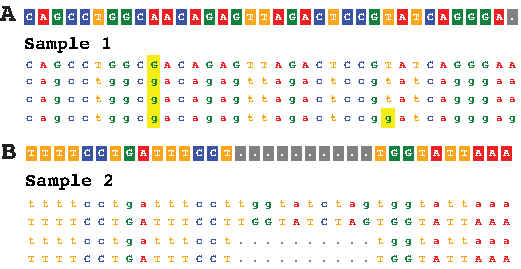
\includegraphics[width=0.5\textwidth]{Figures/App2/Fig1.pdf}
\caption{\textbf{PyBamView display of sequence variants.} In each figure, the reference sequence is shown at the top followed by alignments of each read. Alignments were generated by PyBamView's PDF export feature. \textbf{(a)} Mismatches from the reference sequence, due to either SNPs or sequencing errors, are shown as highlighted bases. \textbf{(b)} Insertions are shown as gaps in the reference, which allows the length and sequence of the insertion to be easily visualized.}
\end{figure}

\section{Example use cases}
Alignment visualization is a critical step of any sequencing experiment. Here I show three examples where PyBamView provides useful visualization of sequence variants. Use cases are not limited to these examples and can theoretically include any ``-seq'' experiment that can be represented by a BAM file.

First, it provides accurate visualizations of different length insertions, such as different alleles of a tandem repeat (\textbf{Supplemental Fig. \ref{fig:pbvsup2}A}). Furthermore, zooming out allows for visualization of large repeat expansions, such as a 60bp CAG expansion in Huntington's Disease (\textbf{Supplemental Fig. \ref{fig:pbvsup2}B}, simulated 250bp reads).

Second, it can be used to analyze variation across samples. This is useful in such analyses as comparing matched tumor vs. normal samples or looking for mutations in affected vs. non-affected individuals in disease genetic studies. (\textbf{Supplemental Fig. \ref{fig:pbvsup3}}) shows example comparisons of individuals at a SNP, small insertion, and a large deletion spanning several kb.

Third, it can visualize complex mutations generated by genome engineering technologies such as CRISPR-Cas9 \cite{CongRanCoxEtAl2013}. Dissecting these mutations requires adequate visualization of indels. An example alignment from a CRISPR library is shown in (\textbf{Supplemental Fig. \ref{fig:pbvsup4}}).

\section{Implementation}
PyBamView is implemented as a Python-based web application using the \href{http://flask.pocoo.org/}{Flask library}. Alignments are processed using a Python backend, which then generates HTML, CSS, and JavaScript files that are displayed in the web browser.

PyBamView takes advantage of BAM and fasta indexing to avoid loading large files into memory. It uses the \href{https://code.google.com/p/pysam/}{pysam} and \href{https://pypi.python.org/pypi/pyfasta/}{pyfasta} libraries for parsing BAM and fasta files, respectively. Both libraries use efficient index data structures, which allow them to quickly fetch data from specific genomic regions of interest. Read alignments are parsed from the CIGAR scores in the BAM file and are displayed  as SVG elements using Javascript. All CIGAR options reported in the SAM specification, including the padded reference option, are supported (\textbf{Supplemental Fig. \ref{fig:pbvsup5}}). 

\section{Conclusion}
As the use of next generation sequencing to analyze complex genomic events grows, there is a critical need for accurate and easy-to-use visualization tools. PyBamView provides a simple yet powerful interface for alignment visualization that facilitates collaborative data analysis.

\section{Acknowledgement} 
The author would like to acknowledge members of the Erlich lab, Alon Goren, and Roy Ronen for helpful feedback, and Assaf Gordon for valuable programming guidance.

This work was supported by a National Defense Science and Engineering Graduate Fellowship [32 CFR 168a].

\section{Supplemental Text}
\label{sec:pbvsuptext}
\subsection{Additional Features}
PyBamView has several features beyond the basic alignment viewer that facilitate specific use cases.
\subsubsection{Pre-defined lists of loci}
A sequencing experiment often targets a specific set of loci. For instance, analysis of STRs may focus on a panel of markers, such as the CODIS set used in forensics or Y-STRs used for genetic genealogy. PyBamView allows the user to provide a bed file containing the coordinates and names of a set of defined loci. The browser view will then show a drop-down box, from which users can easily navigate to loci by name, rather than by genomic coordinate.

\subsubsection{Exporting alignment figures for publication}
Most alignment viewers provide attractive data visualizations, but alignment screenshots are not easily converted to publication-quality figures. PyBamView provides an ``Export snapshot'' option that generates a PDF image of the current alignment. The PDF file can then be easily manipulated by third-party programs to prepare publication-ready figures.

\subsubsection{Serving PyBamView remotely}
PyBamView uses the Python Flask library to launch a web application. Therefore, PyBamView can be served at a URL that is visible remotely to share data with collaborators or as a public resource. To allow viewing PyBamView from a remote computer, add the following arguments:
\begin{itemize}
\item \texttt{-{}-ip 0.0.0.0}: This will allow PyBamView to be accessed on a computer other than the local computer you are running it on.
\item \texttt{-{}-port \$PORT}: where \$PORT is some number between 1024-65535. This must be a port that allows inbound http traffic.
\end{itemize}

For example, if you run:

\texttt{pybamview -{}-bamdir DIRECTORY/WITH/BAMS -{}-ref REF.fa -{}-ip 0.0.0.0 -{}-port 5000}

Then you can navigate to the URL: http://\$MY\_SERVER:5000

where \$MY\_SERVER is either the IP address or hostname of the server from which you are running PyBamView. Detailed usage instructions for serving PyBamView remotely, including how to serve PyBamView using Amazon Web Services, can be found on the usage page of the website (\url{http://mgymrek.github.io/pybamview/usage.html}).

\subsection{Datasets for example use cases}
Sequencing data for the two samples shown in (\textbf{Supplemental Fig. \ref{fig:pbvsup2}}) are from whole genome sequencing of samples HGDP00521 and HGDP00533 available from the Simon's Foundation website at: 
\\
\url{http://www.simonsfoundation.org/life-sciences/simons-human-diversity-project/}.

Sequencing data and variant calls for the samples shown in (\textbf{Supplemental Fig. \ref{fig:pbvsup3}}) were downloaded from the 1000 Genomes Project website (\url{ftp://ftp-trace.ncbi.nih.gov/1000genomes/ftp/}). 

Example CRISPR sequencing data was taken from Hsu et al. \cite{HsuScottWeinsteinEtAl2013}, available as SRA experiment SRP923129 (\url{http://www.ncbi.nlm.nih.gov/bioproject/?term=SRP023129}), run SRR867203. Reads were aligned to hg19 chr2 using BWA \cite{LiDurbin2009} and down-sampled 10,000 fold using Picard's DownsampleSam tool (\url{http://picard.sourceforge.net/command-line-overview.shtml#DownsampleSam}), and were enriched for reads containing evidence of mutations for visualization purposes.

\pagebreak
\section{Supplemental Figures}

\subsection{Supplemental Figure 1}
\begin{figure}[h!]
\centering
\label{fig:pbvsup1}
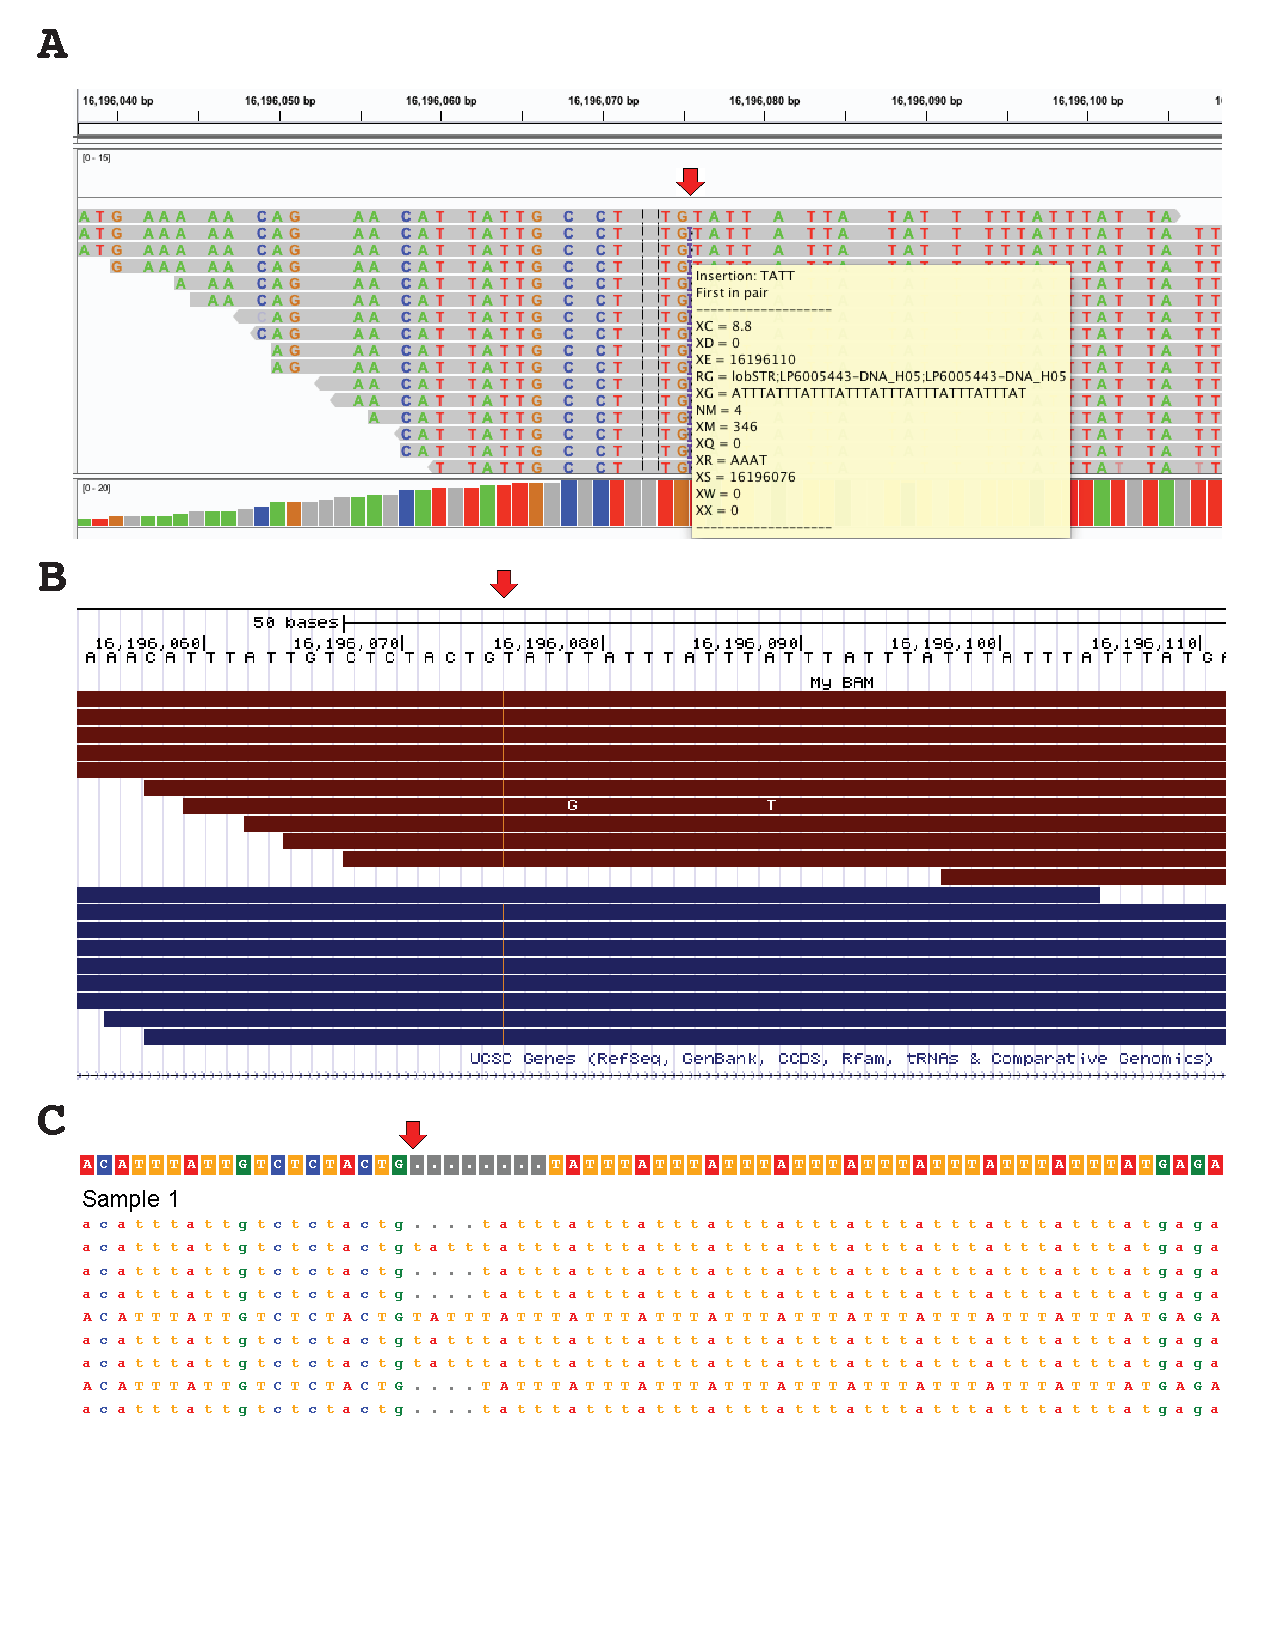
\includegraphics[width=0.65\textwidth]{Figures/App2/SuppFig1.pdf}
\end{figure}
\textbf{Insertion display on current browsers compared to PyBamView.} The alignment shows an individual heterozygous for two alleles with insertions of different lengths from the reference sequence (shown under the red arrows). \textbf{(A)} The Integrative Genomics Viewer (IGV) displays insertions as vertical bars. The user must hover over each variant to see the sequence and length of the insertion. \textbf{(B)} Similarly, the UCSC genome browser displays insertions using an orange line, which does not distinguish between different insertion alleles. \textbf{(C)} PyBamView displays the entire sequence of each insertion, which allows the user to easily visualize the two alleles.

\pagebreak
\subsection{Supplemental Figure 2}
\begin{figure}[h!]
\centering
\label{fig:pbvsup2}
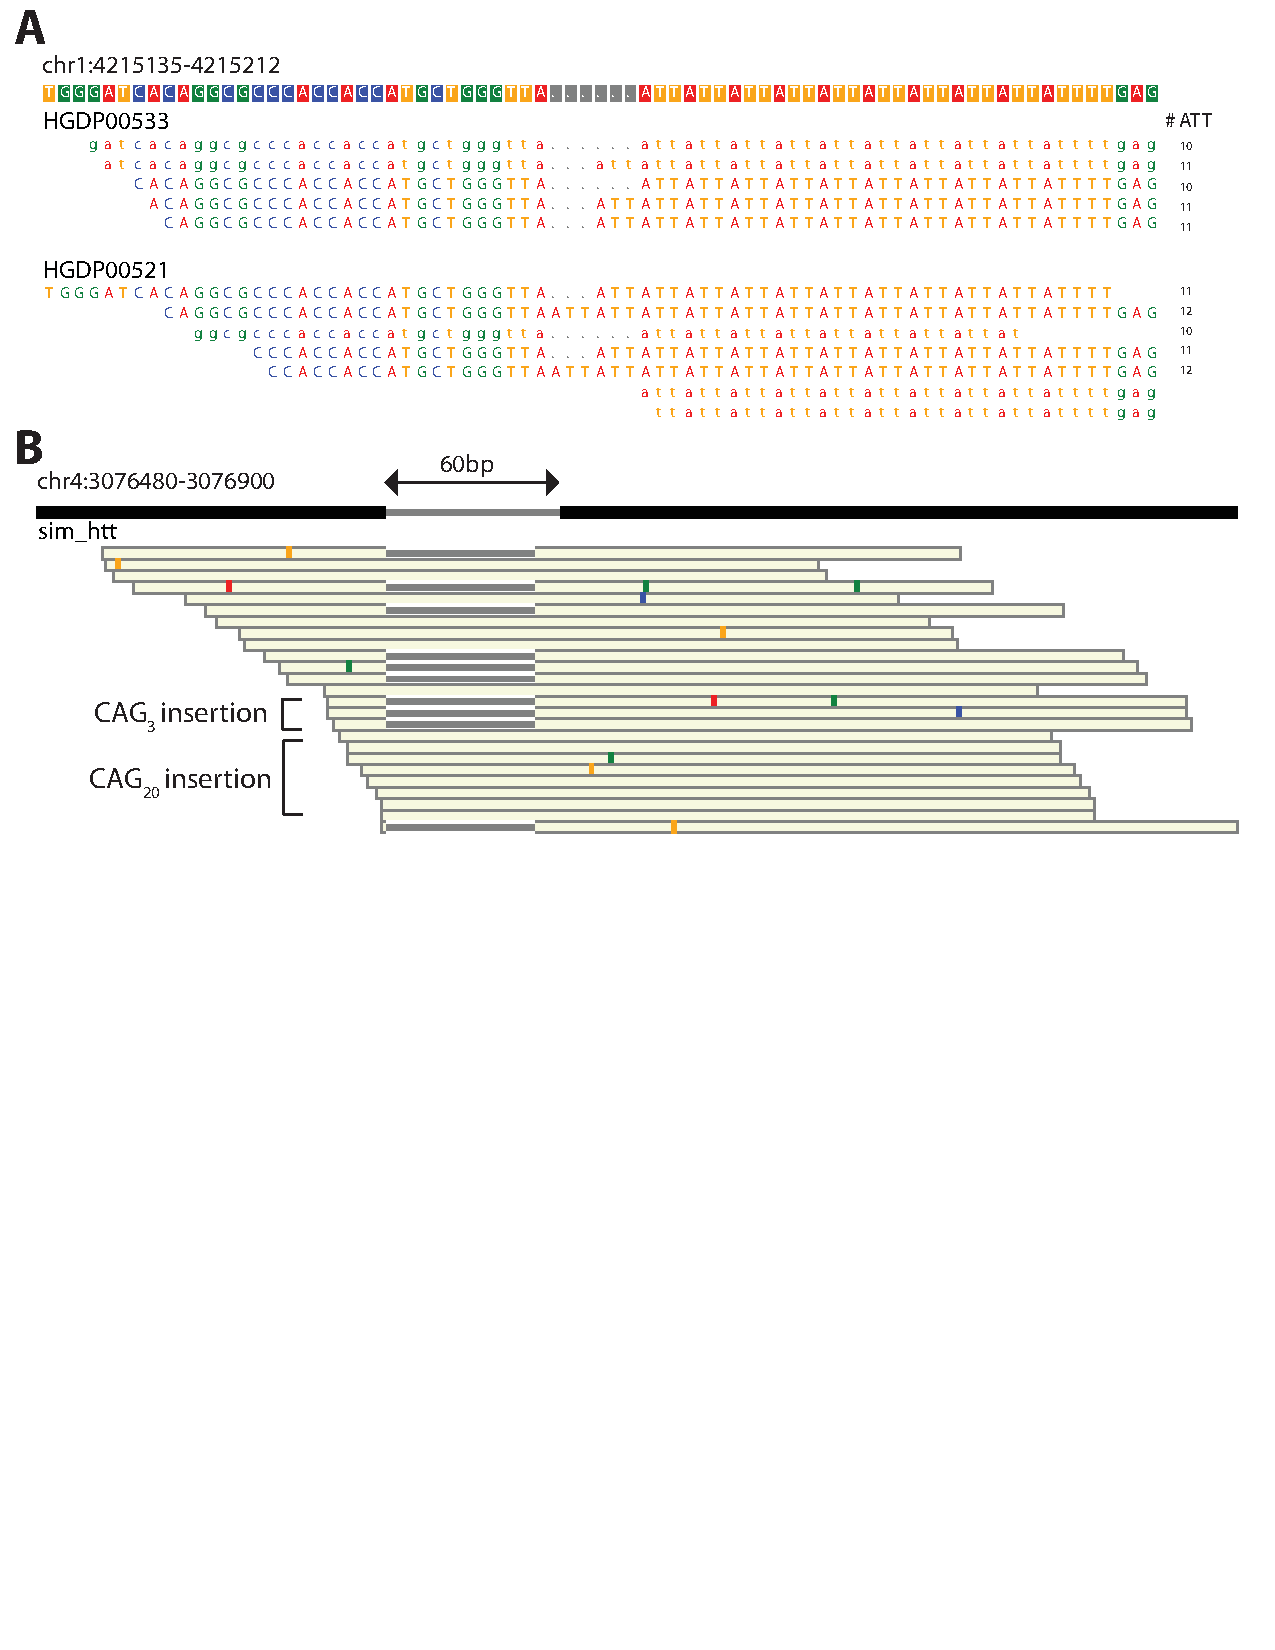
\includegraphics[width=0.65\textwidth]{Figures/App2/SuppFig2.pdf}
\end{figure}
\textbf{Accurate display of short tandem repeat alleles.} \textbf{(A)} Alignments show two distinct short tandem repeat alleles (ATT11 and ATT12) that are longer than the reference allele (ATT10). The allele supported by each read is annotated to the right of the alignment. \textbf{(B)} The padded reference distinguishes between a pathogenic expansion of 60bp vs. a non-pathogenic expansion of 9bp at the CAG trinucleotide repeat implicated in Huntington's Disease. Gaps in the reference sequence and in each read are represented by gray bars. Mismatches from the reference are colored according to the nucleotide of the mismatched base. Example reads supporting each allele are annotated. Data are from simulated 250bp reads with a 0.2\% sequencing error rate. 

\pagebreak
\subsection{Supplemental Figure 3}
\begin{figure}[h!]
\centering
\label{fig:pbvsup3}
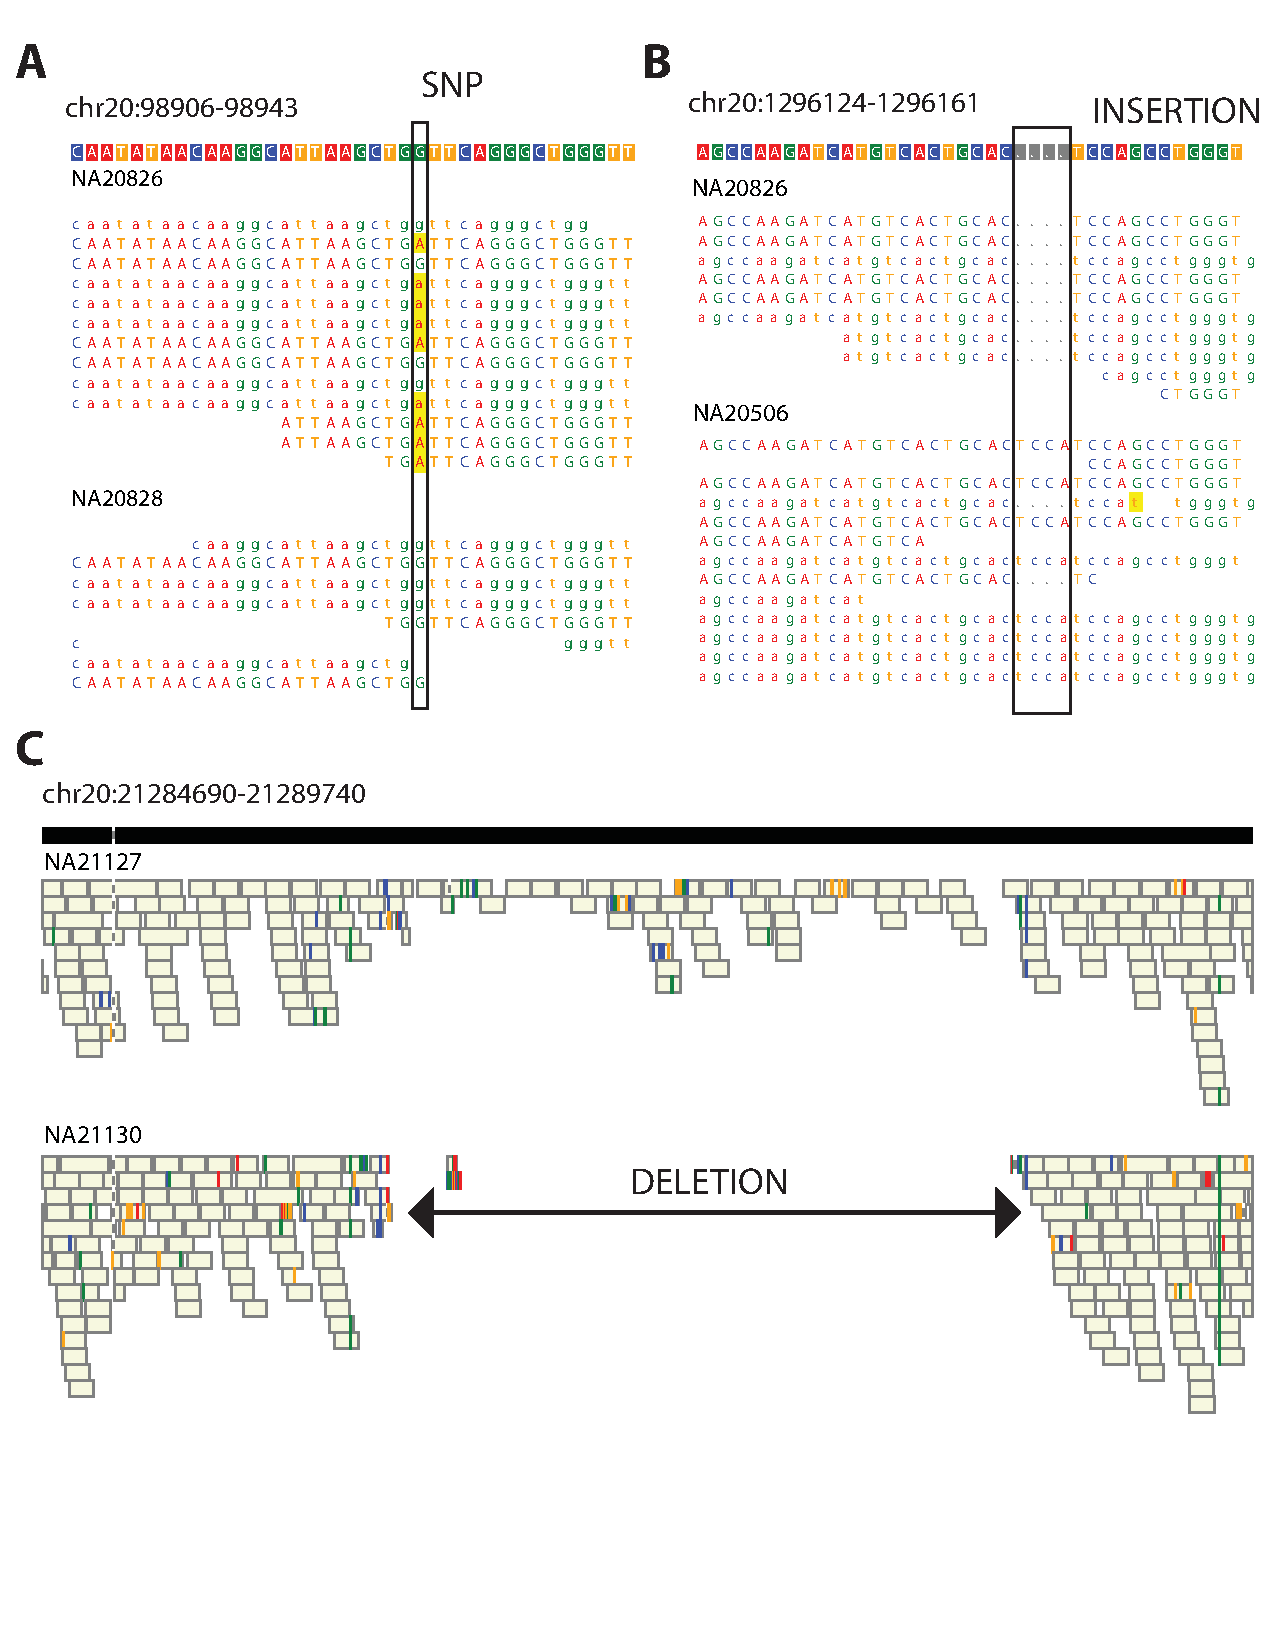
\includegraphics[width=0.65\textwidth]{Figures/App2/SuppFig3.pdf}
\end{figure}
\textbf{Comparing variants between 1000 Genomes Project individuals.} PyBamView allows for visualization of a wide range of variant types across samples. \textbf{(A)} A SNP that is heterozygous in sample NA20826 and homozygous reference in NA20828 is highlighted in yellow. \textbf{(B)} A small insertion that is homozygous reference in NA20826 and heterozygous in NA20506. \textbf{(C)} Zooming out allows visualization of a homozygous large deletion spanning several kb in NA21130 that is heterozygous in NA21127.

\pagebreak
\subsection{Supplemental Figure 4}
\begin{figure}[h!]
\centering
\label{fig:pbvsup4}
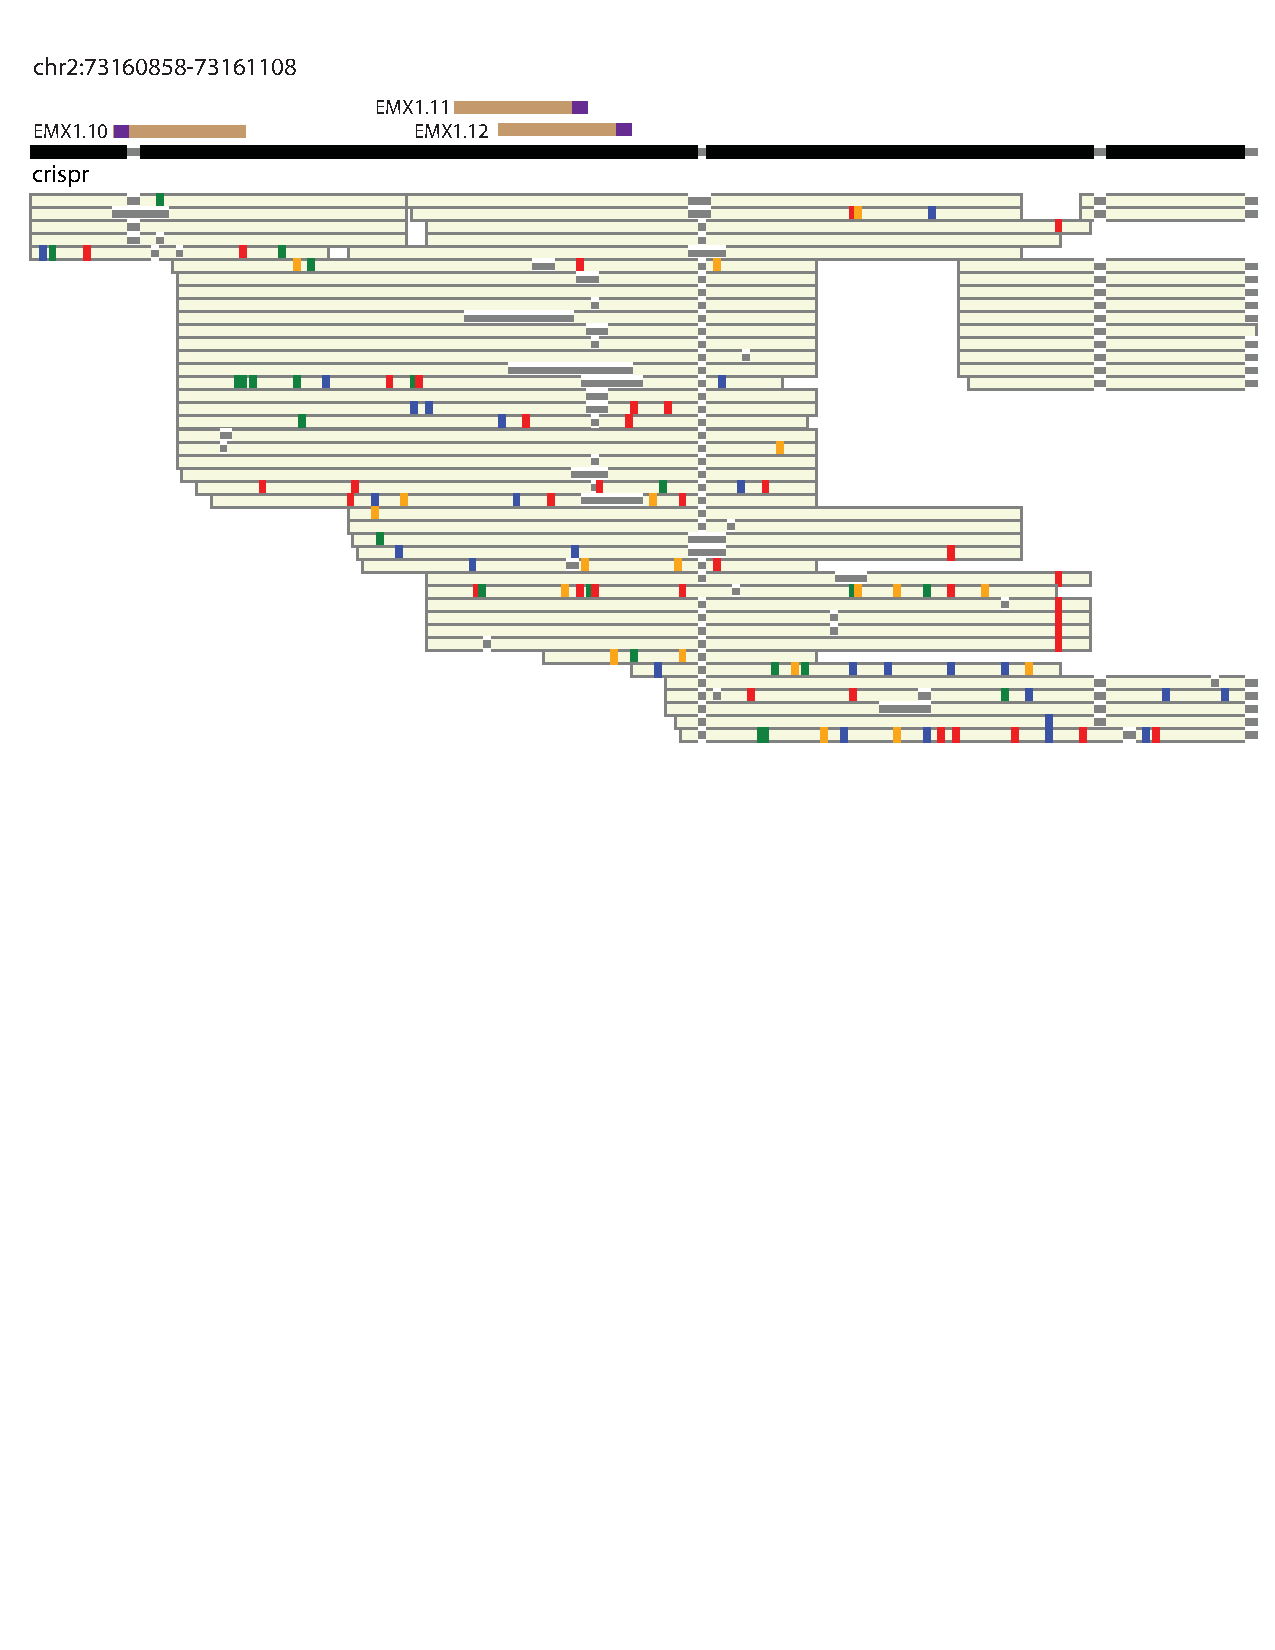
\includegraphics[width=0.65\textwidth]{Figures/App2/SuppFig4.pdf}
\end{figure}
\textbf{Analyzing mutations from genome engineering experiments.} Example sequencing data was obtained from a CRISPR experiment by Hsu et al. \cite{HsuScottWeinsteinEtAl2013} targeting the gene \emph{EMX1}. Reads were down-sampled and enriched for reads containing mutations. Brown bars show the location of target sites, and purple bars show the location of PAM sequences. 

\pagebreak
\subsection{Supplemental Figure 5}
\begin{figure}[h!]
\centering
\label{fig:pbvsup5}
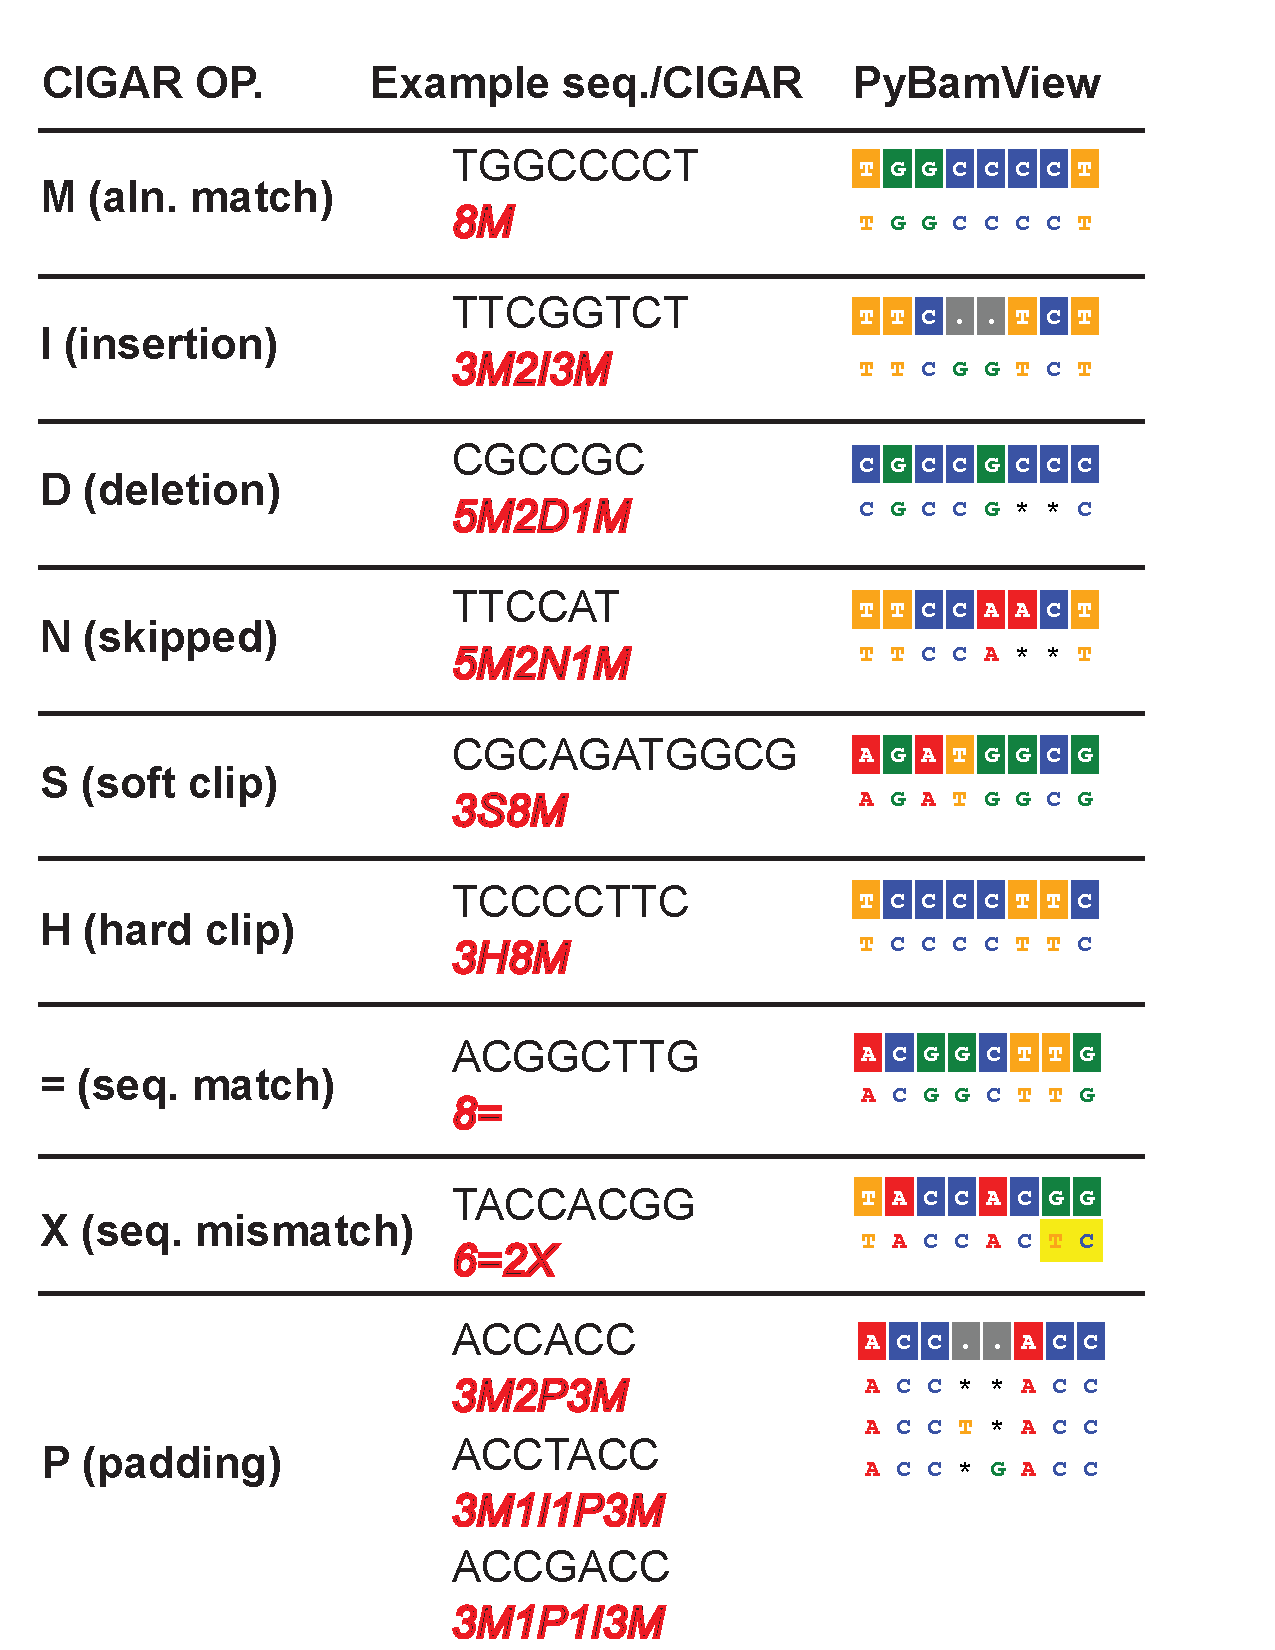
\includegraphics[width=0.65\textwidth]{Figures/App2/SuppFig5.pdf}
\end{figure}
\textbf{PyBamView display of each CIGAR operation.} The first column gives each CIGAR operation supported by the SAM specification. The second column gives an example sequence and corresponding CIGAR score. The third column shows how the reference (top) and read (bottom) sequences are displayed by PyBamView. 



